
Temporal and spatial analysis of five physiographic regions- Tarai, Siwalik, Middle-mountain, and High-mountain and Himalayas of Koshi Basin.

\begin{table}[htbp]
  \centering
  \caption{Spatial distribution of temporal trends of temperature for 1962-2022}
  \begin{tabular}{@{}lcccccc@{}}
      \toprule
      Region & Tmax Trend & Tmax p-value & Tmin Trend & Tmin p-value & Tavg Trend & Tavg p-value \\ 
      \midrule
      \textbf{Himalaya} & & & & & & \\ 
      Monsoon & -0.0111 & 0.1672 & -0.0160 & 0.2340 & -0.0135 & 0.1964 \\ 
      Postmonsoon & 0.0114 & 0.1412 & -0.0011 & 0.9435 & 0.0051 & 0.6504 \\ 
      Premonsoon & \textbf{0.0186*} & 0.0115 & 0.0040 & 0.7977 & 0.0113 & 0.3058 \\ 
      Winter & 0.0031 & 0.7077 & -0.0177 & 0.0972 & -0.0073 & 0.4334 \\ 
      \midrule
      \textbf{High Mountain} & & & & & & \\ 
      Monsoon & -0.0038 & 0.5811 & \textbf{-0.023*} & 0.0019 & \textbf{-0.01*} & 0.0062 \\ 
      Postmonsoon & \textbf{0.0233*} & 0.0035 & 0.0128 & 0.1022 & \textbf{0.02*} & 0.0035 \\ 
      Premonsoon & 0.0125 & 0.0845 & \textbf{0.0164*} & 0.0103 & \textbf{0.01*} & 0.0084 \\ 
      Winter & \textbf{0.0317*} & 0.0058 & -0.0088 & 0.2583 & 0.0114 & 0.1407 \\ 
      \midrule
      \textbf{Middle Mountain} & & & & & & \\ 
      Monsoon & \textbf{-0.0122*} & 0.0338 & \textbf{-0.013*} & 0.0076 & \textbf{-0.01*} & 0.0157 \\ 
      Postmonsoon & 0.0032 & 0.5873 & 0.0011 & 0.8304 & 0.0021 & 0.6808 \\ 
      Premonsoon & 0.0071 & 0.2333 & 0.0074 & 0.1586 & 0.0072 & 0.1738 \\ 
      Winter & -0.0004 & 0.9422 & \textbf{-0.021*} & 0.0002 & \textbf{-0.01*} & 0.0466 \\ 
      \midrule
      \textbf{Siwalik} & & & & & & \\ 
      Monsoon & \textbf{-0.0552*} & 0.0000 & \textbf{-0.06*} & 0.0000 & \textbf{-0.06*} & 0.0000 \\ 
      Postmonsoon & -0.0135 & 0.0945 & \textbf{-0.04*} & 0.0000 & \textbf{-0.03*} & 0.0003 \\ 
      Premonsoon & -0.0106 & 0.1916 & \textbf{-0.04*} & 0.0005 & \textbf{-0.03*} & 0.0017 \\ 
      Winter & \textbf{-0.0260*} & 0.0030 & \textbf{-0.10*} & 0.0000 & \textbf{-0.06*} & 0.0000 \\ 
      \midrule
      \textbf{Tarai} & & & & & & \\ 
      Monsoon & \textbf{-0.0183*} & 0.0005 & -0.0215 & 0.0000 & -0.0199 & 0.0000 \\ 
      Postmonsoon & 0.0027 & 0.5809 & -0.0045 & 0.4620 & -0.0009 & 0.8552 \\ 
      Premonsoon & 0.0067 & 0.2577 & 0.0011 & 0.8275 & 0.0039 & 0.4280 \\ 
      Winter & -0.0006 & 0.9121 & -0.0280 & 0.0000 & -0.0143 & 0.0104 \\ 
      \bottomrule
  \end{tabular}
  \label{tab:spatial_trends}
  \begin{flushleft}
    \footnotesize{* Indicates \( p \leq 0.05 \) which denotes significant changes} \\
    
\end{flushleft}
\end{table}




Table\ref{tab:spatial_trends} presents the regional and seasonal distribution of temperature trends across the Koshi Basin. In the Himalaya region, the Pre-monsoon season shows a statistically significant warming trend in Tmax (0.0186, p=0.0115), indicating potential shifts in climatic patterns that may affect the region’s ecosystem. Conversely, the Monsoon season reflects slight cooling trends in Tmax (-0.0111, p=0.1672) and Tmin (-0.0160, p=0.2340). The High Mountain region exhibits diverse temperature trends, with the post-monsoon season showing a significant warming trend for Tmax (0.0233, p=0.0035) and Tavg (0.0181, p=0.0035). The Pre-monsoon season also indicates a notable warming trend in Tmax (0.0125, p=0.0845), while Tmin trends remain relatively stable. The Middle Mountain region presents a more mixed scenario. The Monsoon season reveals a significant cooling trend in Tmax (-0.0122, p=0.0338) and Tmin (-0.0128, p=0.0076). The other seasons show minimal or non-significant trends, indicating that temperature variability is more pronounced during the Monsoon. In the Siwalik region, stark cooling trends are evident across all seasons, particularly during the Monsoon (-0.0552, p=0.0000) and Winter (-0.0260, p=0.0030) seasons. The extreme cooling in Tmax (-0.0572, p=0.0000) and Tmin (-0.0592, p=0.0000). the Tarai region demonstrates notable cooling trends during the Monsoon (-0.0183, p=0.0005) and Winter (-0.0280, p=0.0000) seasons. The Tmin trends in the Monsoon are also significant (-0.0215, p=0.0000). These findings point to unique seasonal and regional differences in Nepal's temperature changes.


The study conducted by \citet{shrestha_climate_2011} discovered regular warming trends in seasonal mean maximum temperatures in all of Nepal's regions during 1977 to 1994, with warming seen throughout the winter, pos-monsoon, pre-monsoon, and monsoon seasons. On the other hand, the present study's seasonal analysis reveals more diversified tendencies: the Hills and Middle Mountains show mixed trends, with major drops in Tmin during Monsoon and Winter, while the High Mountains show minimal changes with a significant Tmax rise mainly during Pre-monsoon. Significant seasonal cooling tendencies are visible in the Siwalik and Tarai areas, especially during the Monsoon and Winter, indicating different regional temperature behaviors from previous research. \citet{shrestha_observed_2017} observed long-term trends (1975--2010) in seasonal maximum and minimum temperatures showed an overall increase at most stations, though some decreases were observed in winter and pre-monsoon. Seasonal minimum temperatures increased more than maximum temperatures. The findings indicated widespread significant warming, particularly in indices based on daily minimum temperatures, with stronger warming trends in more recent decades. Study  by \citet{nayava_spatial_2017} for 1981--2010 shows varying seasonal temperature trends across Nepal. In the Terai, Valley, Hill, Mountain regions warming is presence across all season from 0.01-0.13°C/year, whereas the Trans-Himalaya shows 0.03°C in pre-monsoon, -0.02°C in post-monsoon, 0.01°C in monsoon, and 0.08°C in winter.


Similarly \citet{shrestha_maximum_1999} for 1977 to 1994, temperature trends across Nepal showed significant regional and seasonal variation, with the Trans-Himalaya experiencing the highest winter warming at 0.124°C/year, the Middle Mountains seeing the largest monsoon increase at 0.094°C/year, and the post-monsoon season showing an overall national average warming rate of 0.059°C/year, while the Terai region exhibited a much lower warming rate of 0.006°C/year in winter and -0.004°C/year in pre-monsoon.

\begin{figure}[H] 
  \centering
  \includegraphics[width=0.9\textwidth]{images/simple_plots_Premonsoon_Trend.png}  
  \caption{Pre-monsoon temperature trends across the time intervals (a) 1962–1971, (b) 1972–1981, (c) 1982–1991, (d) 1992–2001, (e) 2002–2011, (f) 2012–2021, and (g) 1962–2022.} 
  \label{fig:Pre-monsoon temperature trends}  
\end{figure}

\begin{figure}[H] 
  \centering
  \includegraphics[width=0.9\textwidth]{images/simple_plots_Monsoon_Trend.png}  
  \caption{Monsoon temperature trends across the time intervals (a) 1962–1971, (b) 1972–1981, (c) 1982–1991, (d) 1992–2001, (e) 2002–2011, (f) 2012–2021, and (g) 1962–2022.} 
  \label{fig:Monsoon temperature trends}  
\end{figure}

\begin{figure}[H] 
  \centering
  \includegraphics[width=0.9\textwidth]{images/simple_plots_Postmonsoon_Trend.png}
  \caption{Post-monsoon temperature trends across the time intervals (a) 1962–1971, (b) 1972–1981, (c) 1982–1991, (d) 1992–2001, (e) 2002–2011, (f) 2012–2021, and (g) 1962–2022.} 
  \label{fig:Post-monsoon temperature trends}  
\end{figure}

\begin{figure}[H] 
  \centering
  \includegraphics[width=0.9\textwidth]{images/simple_plots_Winter_Trend.png}  
  \caption{Winter temperature trends across the time intervals (a) 1962–1971, (b) 1972–1981, (c) 1982–1991, (d) 1992–2001, (e) 2002–2011, (f) 2012–2021, and (g) 1962–2022.} 
  \label{fig:Winter temperature trends}  
\end{figure}

Figures\ref{fig:Pre-monsoon temperature trends, fig:Monsoon temperature trends,fig:Post-monsoon temperature trends,fig:Winter temperature trends}  present an analysis of temperature trends based on three key factors: temperature type (Tavg, Tmax, Tmin), geographic regions (Himalayas, High Mountain, Middle Mountain, Siwalik, Tarai, and Koshi Basin), and seasonal classifications (Monsoon, Post-monsoon, Pre-monsoon, Winter, and annual trends) across different decades. The temperature trends exhibit considerable variability influenced by the decade, temperature type, physiographic regions, and seasonal characteristics.


Figure\ref{fig:Pre-monsoon temperature trends}, the Pre-monsoon season reveals overall cooling trends in the 1962-1971 decade except in Himalaya regions, similar cooling trend from 1972 to 1981, and later decade experience a warming trend except maximum and average temperature shows cooling trend in 2012-2021.  For the overall period from 1962 to 2022, only the Siwalik region demonstrates a cooling trend; all other regions display warming trends, particularly the Himalayan region, which shows a higher rate of warming at 0.02°C/year.

Figure\ref{fig:Monsoon temperature trends} illustrates that during the Monsoon season, temperature fluctuations have accelerated in recent decades, particularly from 2012 to 2021, with significant warming observed in average and minimum temperatures, while maximum temperatures predominantly show a cooling trend. Overall, from 1962 to 2022, the Monsoon season reflects a cooling trend across the various regions.

Figure\ref{fig:Post-monsoon temperature trends} highlights a cooling trend in the Post-monsoon period from 1962 to 1981, followed by a notable warming trend that has intensified in recent decades.

Figure\ref{fig:Winter temperature trends} indicates distinct temperature trends during the Winter season across different regions and time periods. Minimum and average temperatures experienced warming between 1982-1991 and 2012-2021, while a cooling trend was observed from 1962 to 1971. Maximum temperatures warmed during the 1992-2001 and 2002-2011 decades, with a notable cooling trend of 0.52 degrees Celsius in the High Mountain region from 2012 to 2021. Overall, from 1962 to 2022, the Siwalik region shows a general cooling trend, whereas only the High Mountain region exhibits a warming trend.

\citet{adhikari_x_2016}Adhikari and Devkota (2016) studied temperature trends from 1988 to 2010 in the Annapurna, Langtang, and Khumbu basins. In the Khumbu region, moderate warming was observed across all seasons, with maximum temperatures rising by 0.0857°C/year in winter and 0.0628°C/year in pre-monsoon. Minimum temperatures showed slight changes, with a small increase of 0.0101°C/year in spring and a decrease of -0.0024°C/year during monsoon. Overall, mean temperatures increased by 0.0857°C/year in winter, with Khumbu showing lower trends compared to Langtang and Annapurna, particularly in minimum temperatures.

\begin{figure}[H] 
  \centering
  \includegraphics[width=0.9\textwidth]{images/simple_plots_annual_Trend.png}  
  \caption{Annual temperature trends across the time intervals (a) 1962–1971, (b) 1972–1981, (c) 1982–1991, (d) 1992–2001, (e) 2002–2011, (f) 2012–2021, and (g) 1962–2022.} 
  \label{fig:Annual temperature trends}  
\end{figure}

Figure\ref{fig:Annual temperature trends} illustrates the annual temperature trends across different regions of the Koshi Basin reveal significant variations over the decades. The first two decades (1962--1981) exhibit an overall cooling trend, with the exception of warming observed in the Himalayan regions, where maximum temperatures increased by 0.02 °C and minimum temperatures rose by 0.04 °C in later decades. The period from 1982 to 2021 predominantly shows a warming trend; however, from 2002 to 2011, the Siwalik region experienced a cooling trend, and in 2012 to 2021, maximum temperatures again exhibited a cooling trend. Study conducted by Bajracharya et al., (2023) indicates an increase in projected average temperature across Koshi basin, with higher rates in northern regions. \citet{shrestha_observed_2017} Shrestha et al., (2017) observed a clear warming trend in maximum and minimum temperatures over the Transboundary Koshi basin from 1975 to 2010, with notable spatial variation. Stations in the hills and mountains exhibited significant warming, while in the plains, maximum temperatures showed a decreasing trend. In the Koshi region, the maximum temperature rose at a rate of 0.058 °C per year, while the minimum temperature increased by 0.014 °C per year over the forty years leading up 1963 to 2009 \citep{nepal_impacts_2016} (Nepal, 2016). Similar studies done by \citet{chand_trend_2019} Chand et al., (2019) at Narayani Basin showed that, The annual average temperature is in a decreasing trend till 1972 and increasing order for later years.  Study done by \citet{nayava_spatial_2017} Nayava et al., (2017) shows air temperature trends at different altitudinal zones of Nepal based on 30 years (1981--2010) annual mean temperatures increased at varying rates, with the Terai warming by 0.024°C/year, valley floors at 0.034°C/year, hill valleys at 0.063°C/year, mountain valleys at 0.033°C/year, hilltops at 0.072°C/year, mountain tops at 0.038°C/year, and the Trans-Himalaya at 0.029°C/year. \citet{paudel_climate_2021}Paudel et al., (2021) found that between 1980 and 2018, the mean annual temperature in the transboundary Koshi River Basin increased by 0.084°C/year in the mountains, 0.0975°C/year in the hills, and 0.0187°C/year in the Tarai. Study done by \citet{shrestha_maximum_1999} Shrestha et al., (1999) for annual temperature trends from 1977 to 1994 revealed that the Trans-Himalaya experienced the most significant warming at 0.090°C/year. The Himalaya and Middle Mountains also showed substantial warming, with trends of 0.057°C/year and 0.075°C/year, respectively. Siwalik and Terai regions had the lowest annual temperature trends, both at 0.041°C/year. The all-Nepal average annual warming rate was 0.059°C/year, showing widespread temperature increases across the country. \citet{adhikari_x_2016} Adhikari and Devkota, (2016) observed annual temperature trends in the Khumbu region from 1988 to 2010. The maximum temperature increased by 0.0639°C/year, while the minimum temperature showed a slight rise of 0.0036°C/year. Overall, the mean annual temperature in Khumbu increased by 0.0639°C/year.


\begin{table}[htbp]
  \centering
  \caption{Regional temperature regression equations}
  \begin{tabular}{@{}lccc@{}}
      \toprule
      \textbf{Region} & \textbf{Tmin Equation} & \textbf{Tmax Equation} & \textbf{Tavg Equation} \\ 
      \midrule
      Himalaya & \( y = -0.01x + 15.46 \) & \( y = 0.00x + 2.58 \) & \( y = -0.00x + 9.02 \) \\ 
      High Mountain & \( y = -0.00x + 13.97 \) & \( y = 0.01x - 9.35 \) & \( y = 0.00x + 2.31 \) \\ 
      Middle Mountain & \( y = -0.01x + 27.88 \) & \( y = -0.00x + 27.81 \) & \( y = -0.00x + 27.85 \) \\ 
      Siwalik & \( y = -0.06x + 145.24 \) & \( y = -0.03x + 91.55 \) & \( y = -0.05x + 118.40 \) \\ 
      Tarai & \( y = -0.01x + 50.79 \) & \( y = -0.00x + 41.15 \) & \( y = -0.01x + 45.97 \) \\ 
      \bottomrule
  \end{tabular}
  \label{tab:regression_equations}
\end{table}




\begin{table}[H]
  \centering
  \caption{Nonparametric (Mann-Kendall Test) tests for annual regional trends for the period 1962–2022}
  \begin{tabular}{@{}lccc@{}}
      \toprule
      \textbf{Regions} & \textbf{Tmin Slope} & \textbf{Tmax Slope} & \textbf{Tavg Slope} \\ 
      \midrule
      Himalaya        & -0.009       & 0.005**      & -0.000** \\ 
      High Mountains  & -0.016       & 0.008**      & 0.002**  \\ 
      Middle Mountains & -0.008      & -0.001**     & -0.003** \\ 
      Siwalik         & -0.063       & -0.033       & -0.05    \\ 
      Tarai           & -0.015       & -0.003**     & -0.006** \\ 
      \bottomrule
  \end{tabular}
  \label{tab:mann_kendall}
  \begin{flushleft}
    \footnotesize{** indicates $p \geq 0.05$ which denotes no significant changes.}
\end{flushleft}
  \caption*{** indicates $p \geq 0.05$ which denotes no significant changes.}
\end{table}



The Annual Regional Mann-Kendall test findings are shown in the table~\ref{tab:mann_kendall}.

This test evaluates trends in minimum (\(T_{\text{min}}\)), maximum (\(T_{\text{max}}\)), and average (\(T_{\text{avg}}\)) temperatures in five regions: Tarai, Siwalik, Middle Mountains, High Mountains, and Himalaya. While \(T_{\text{max}}\) and \(T_{\text{avg}}\) show rising tendencies (0.005** and -0.000**, respectively) in the Himalaya, the \(T_{\text{min}}\) shows a decreasing trend (-0.009), and the latter two are not statistically significant (\(p \geq 0.05\)). \(T_{\text{min}}\) and \(T_{\text{avg}}\) (-0.008 and -0.003**) also exhibit declining patterns in the Middle Mountain region, although \(T_{\text{max}}\) (-0.001**) shows a relatively constant trend. The High Mountains, on the other hand, show an increasing trend in \(T_{\text{min}}\) (-0.016) and a more marked reduction in \(T_{\text{max}}\) and \(T_{\text{avg}}\) (0.008** and 0.002**). All temperature measurements exhibit similar declines in the Siwalik region: \(T_{\text{min}}\) (-0.063), \(T_{\text{max}}\) (-0.033), and \(T_{\text{avg}}\) (-0.05). Lastly, with \(T_{\text{min}}\) (-0.015), \(T_{\text{max}}\) (-0.003**), and \(T_{\text{avg}}\) (-0.006**) showing diminishing trends across all temperature parameters, the Tarai also shows declining trends, but \(T_{\text{max}}\) and \(T_{\text{avg}}\) are not statistically significant. Similarly, the Koshi region's maximum temperature grew at a rate of 0.058 °C/year, and its minimum temperature increased at a rate of 0.014 °C/year during the forty years leading up to 1963–-2009~\citep{nepal_impacts_2016}.





\begin{figure}[htbp]
  \centering
  \begin{subfigure}{0.45\textwidth}
      \centering
      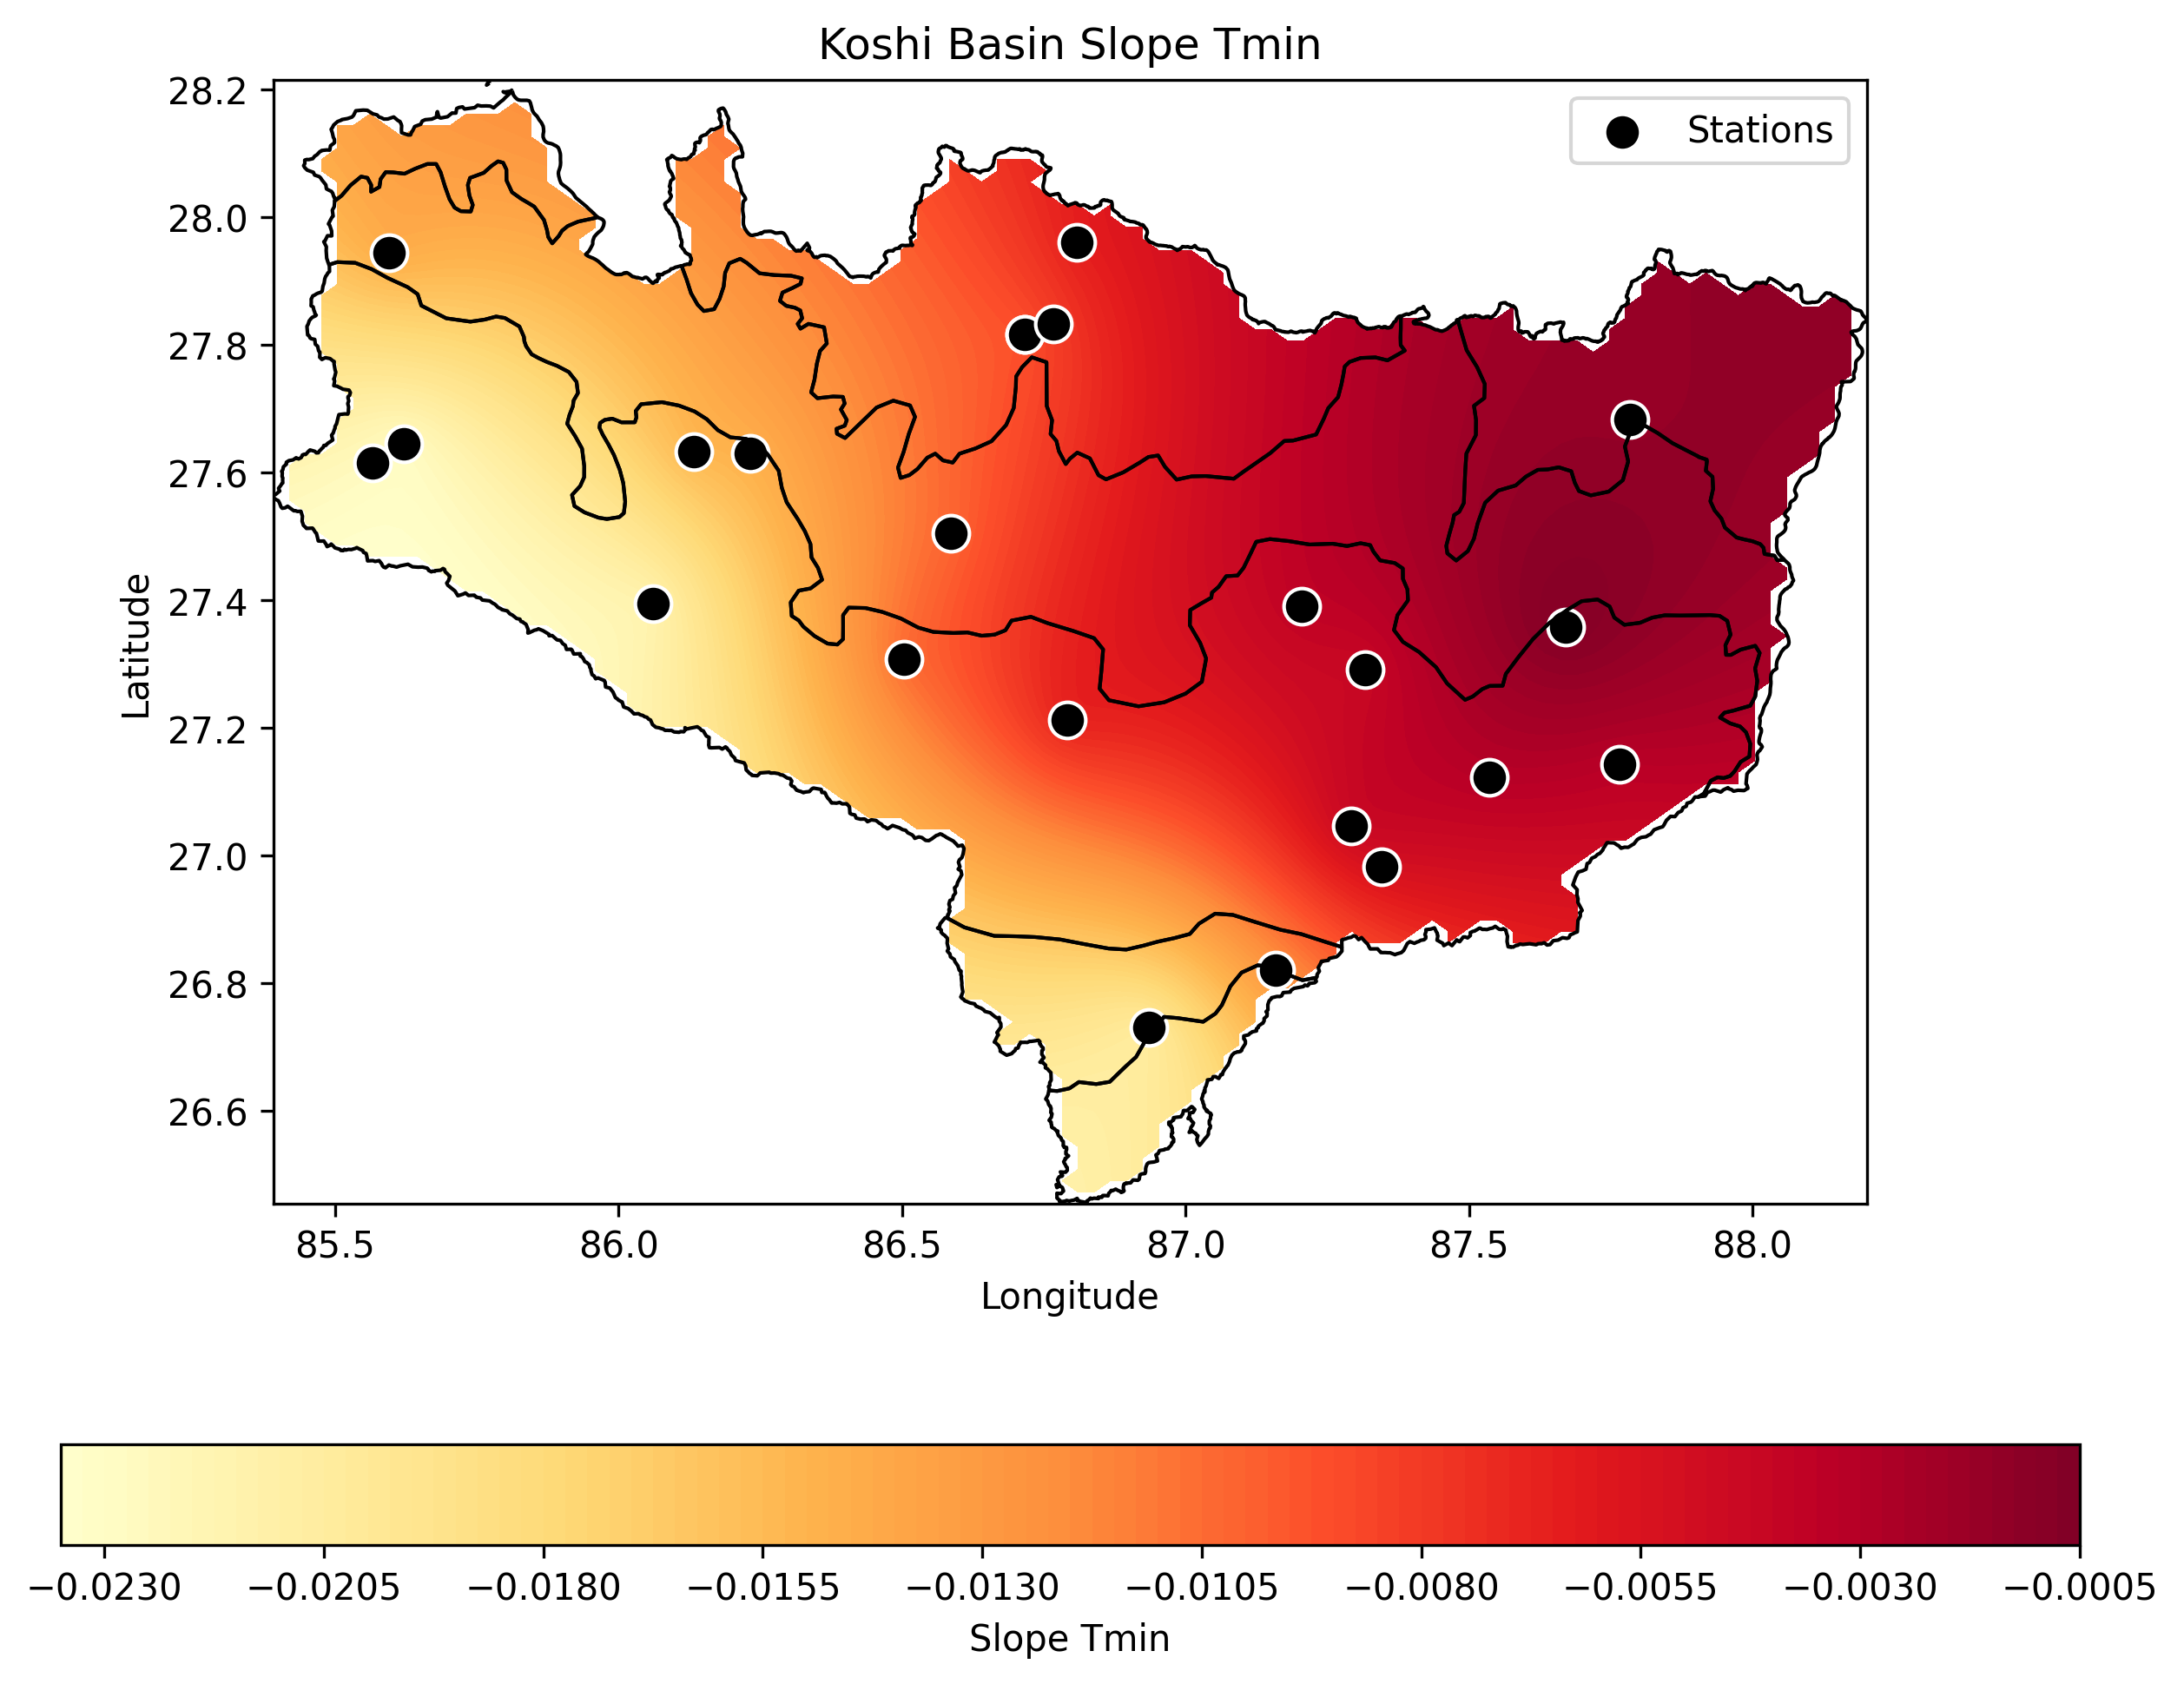
\includegraphics[width=\linewidth]{images/avg_krig_Koshi Basin Slope Tmin.png}
      \caption{Caption for subfigure (a)}
      \label{fig:7a}
  \end{subfigure}
  \hfill
  \begin{subfigure}{0.45\textwidth}
      \centering
      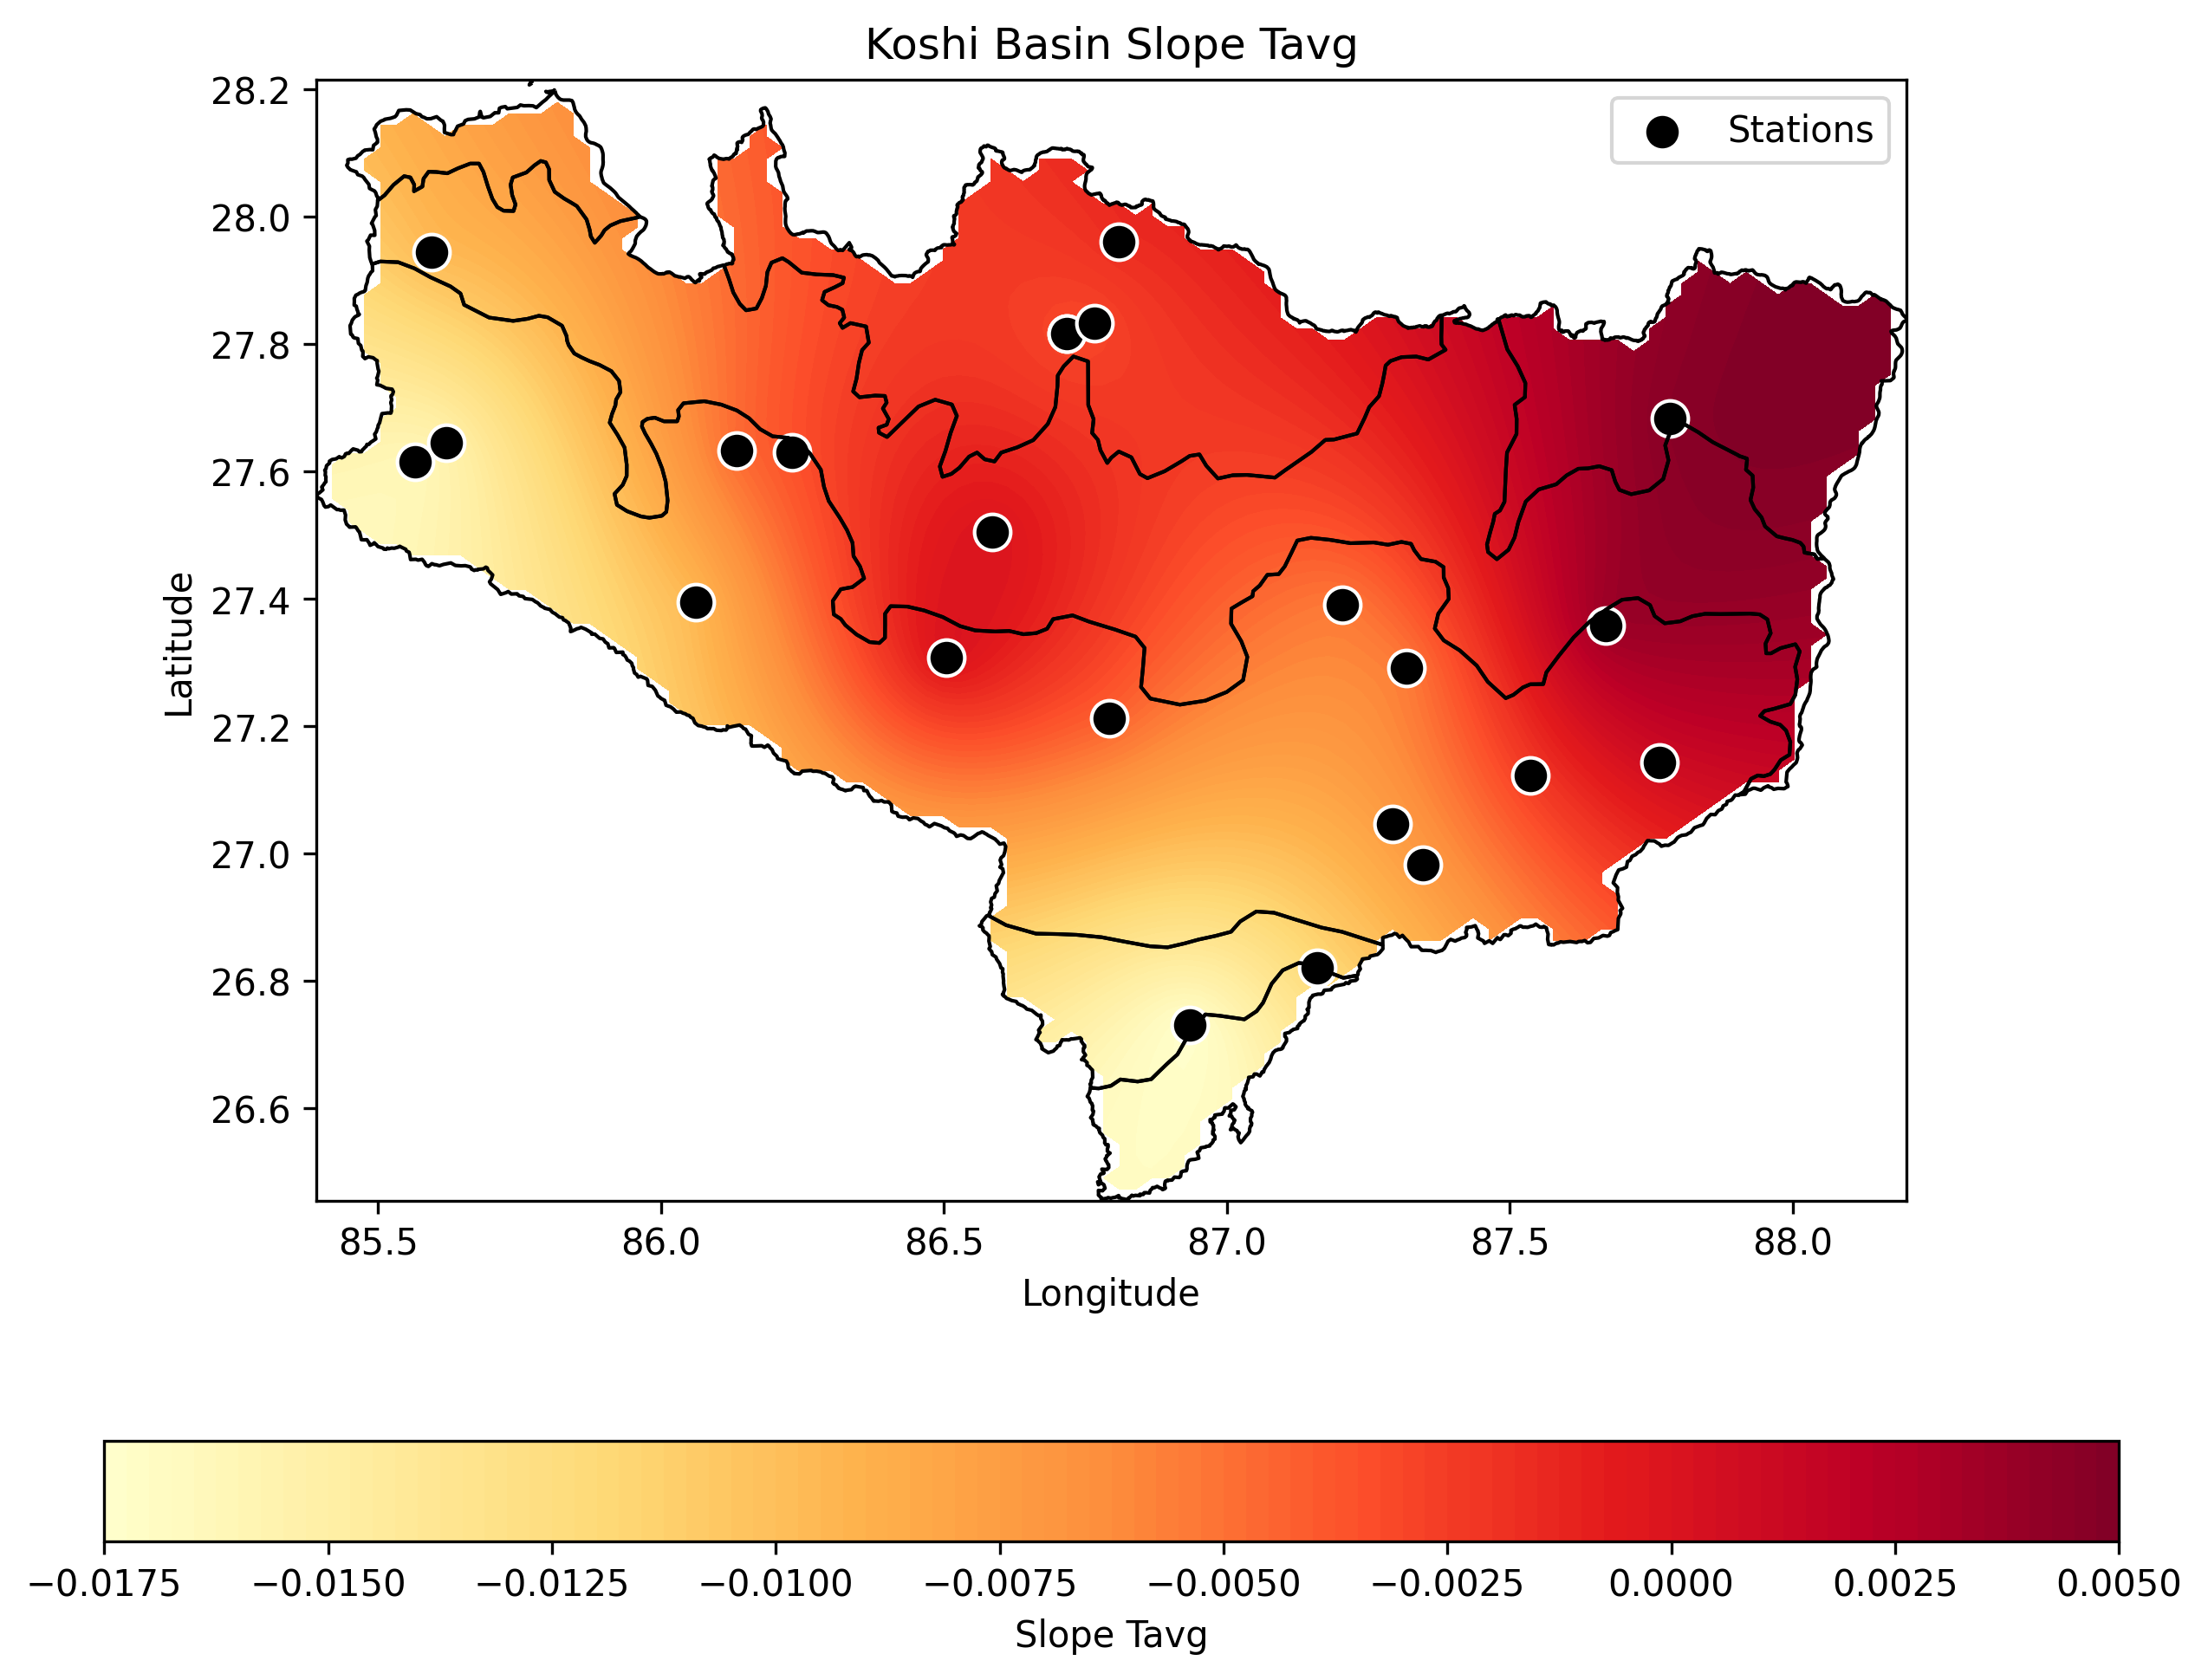
\includegraphics[width=\linewidth]{images/avg_krig_Koshi Basin Slope Tavg.png}
      \caption{Caption for subfigure (b)}
      \label{fig:7b}
  \end{subfigure}
  
  \vspace{0.5cm} % Adjust space between rows as needed
  
  \begin{subfigure}{0.45\textwidth}
      \centering
      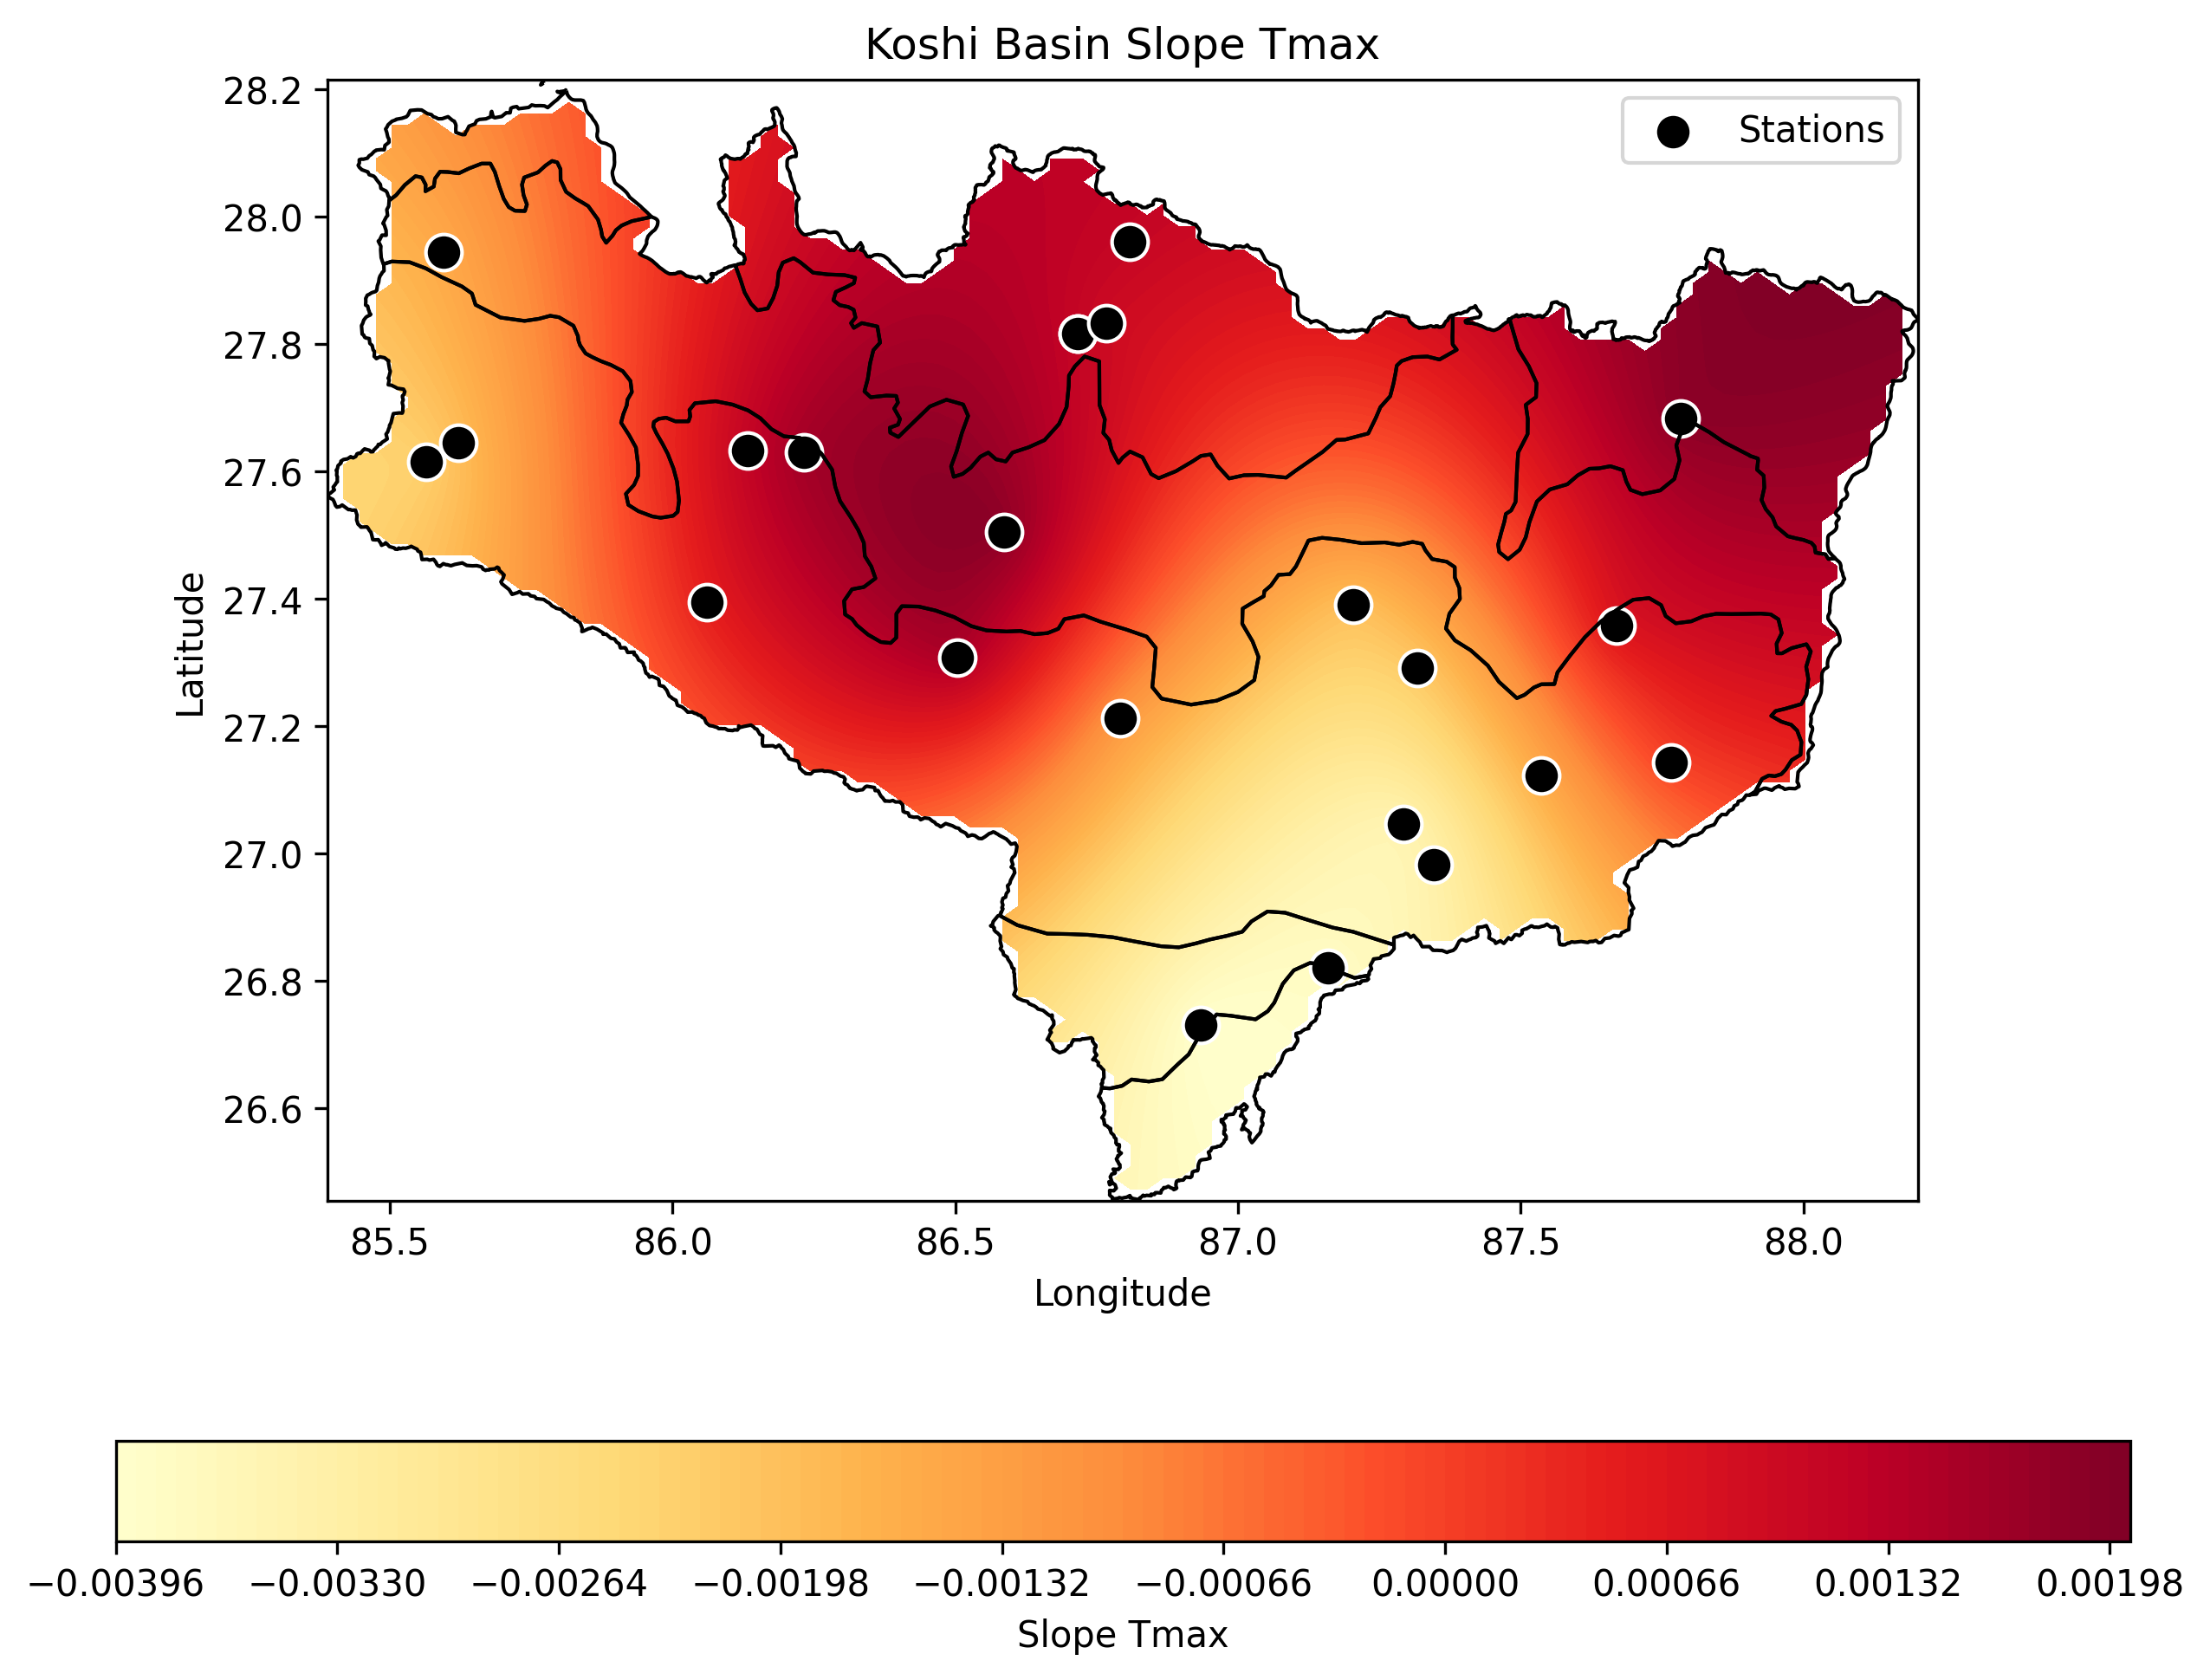
\includegraphics[width=\linewidth]{images/avg_krig_Koshi Basin Slope Tmax.png}
      \caption{Caption for subfigure (c)}
      \label{fig:7c}
  \end{subfigure}
  
  \caption{Spatial distributions of annual temperature trends for the period 1962–2022 for (a) Tmin, (b) Tavg, (c) Tmax}
  \label{fig:krig_results}
\end{figure}


Figure~\ref{fig:krig_results} illustrates a nonuniform temperature trend across the Koshi basin region. In Figure 7a, the annual average of daily minimum temperatures shows an overall cooling trend, ranging from -0.0005°C to -0.023°C, with higher elevations experiencing less cooling. In Figure 7b, the annual average temperatures reveal both warming and cooling trends, ranging from -0.0175°C to 0.005°C, where higher elevations tend to warm or cool less compared to the Tarai and Siwalik regions. Similarly, in Figure 7c, the annual average of daily maximum temperatures shows trends from cooling to slight warming, ranging from -0.00396°C to 0.00198°C, with Tmax exhibiting a warming trend in higher elevation areas. Study conducted by \citep{paudel_climate_2021} in transboundary Koshi basin for the data between 1980 and 2018, the mean annual temperature in the Koshi River Basin increased by 0.084°C/ year in the mountain region (p = 0.0005), 0.0975°C/year in the hill region (p = 0.0002), and 0.0187°C/year in the Tarai region (p = 0.0206), with significant correlations throughout.  illustrates a nonuniform temperature trend across the Koshi basin region. In Figure 7a, the annual average of daily minimum temperatures shows an overall cooling trend, ranging from -0.0005°C to -0.023°C, with higher elevations experiencing less cooling. In Figure 7b, the annual average temperatures reveal both warming and cooling trends, ranging from -0.0175°C to 0.005°C, where higher elevations tend to warm or cool less compared to the Tarai and Siwalik regions. Similarly, in Figure 7c, the annual average of daily maximum temperatures shows trends from cooling to slight warming, ranging from -0.00396°C to 0.00198°C, with Tmax exhibiting a warming trend in higher elevation areas. Study conducted by \citet{paudel_climate_2021} in transboundary Koshi basin for the data between 1980 and 2018, the mean annual temperature in the Koshi River Basin increased by 0.084°C/ year in the mountain region (p = 0.0005), 0.0975°C/year in the hill region (p = 0.0002), and 0.0187°C/year in the Tarai region (p = 0.0206), with significant correlations throughout. 

